%!Tex Root = ../main.tex
% ./Packete.tex
% ./Design.tex
% ./Deklarationen.tex
% ./Vorbereitung.tex
% ./Aufgabe2.tex
% ./Aufgabe3.tex
% ./Aufgabe4.tex
% ./Appendix.tex

\section{Aufgabe 1}

\setcounter{exercise}{1}

\begin{frame}[allowframebreaks]{Aufgabe \thesection}{Betrag Zweierkomplementzahl}

\begin{exercisenoinc}
Entwickle einen Schaltkreis zu:\\
$$abs_n\ :\ \mathbb{B}^n\rightarrow\mathbb{B}^n, (a_{n-1},...,a_0)\mapsto (s_{n-1},...,s_0)$$
$$\langle s_{n-1},...,s_0\rangle = |[a_{n-1},...,a_0]|$$
\end{exercisenoinc}

% \begin{requirementsnoinc}
%     $[]$ steht für 2er-Komplement, $\langle\rangle$ ist die \dq klassische\dq\ Binär-Interpretation.\\
% \end{requirementsnoinc}

\begin{solutionnoinc}
    \center 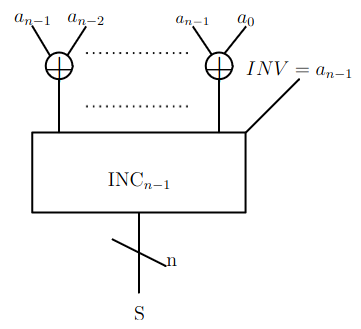
\includegraphics[width=150pt]{figures/Absolute.png}
\end{solutionnoinc}

\begin{solutionnoinc}
    $cost(abs_n)=cost(INC_n-1)+(n-1)\cdot cost(XOR)=(n-1)\cdot cost(HA)+(n-1)$\\ $\qquad\qquad\ \ =3(n-1)$\\\ \\
    Es gibt \textbf{keinen} Überlauf!\quad $|[10...0]|= \langle 10...0\rangle$
\end{solutionnoinc}

\end{frame}
